%% jbc-template.tex, version 1.0, 2016/08/16
\documentclass[alpha-refs]{wiley-article}
% \documentclass[blind,num-refs]{wiley-article}

% Add additional packages here if required
\usepackage{siunitx}

% Update article type if known
\papertype{Original Article/ Review?}
% Include section in journal if known, otherwise delete
\paperfield{Methods & Resources}
\usepackage{graphicx}

% These packages can be used!
\usepackage{amsmath,amssymb,mathtools}
\usepackage[version=3]{mhchem}
\usepackage{siunitx}
\usepackage[colorlinks=true, allcolors=blue]{hyperref}

\title{Batch effects in large-scale proteomics studies: diagnostics and correction}

\author[1, 2, 3]{Jelena Čuklina}
\author[1]{Chloe Lee}
\author[1]{Evan G. Williams}
\author[1]{Tatjana Sajic}
\author[1\authfn{2}]{Ben C. Collins}
\author[3]{Maria Rodriguez-Martinez}
\author[2]{Varun Sharma}
\author[1, 4]{Patrick Pedrioli}
\author[1, 5]{Ruedi Aebersold}

\affil[1]{Institute of Molecular Systems Biology, ETH Zurich, Zurich, CH-8093, Switzerland}
\affil[2]{PhD Program in Systems Biology, University of Zurich and ETH Zurich, Zurich, CH-8057  Switzerland}
\affil[3]{IBM Zurich Research Laboratory, Rüschlikon, CH-8803, Switzerland}
\affil[4]{ETH Zürich, PHRT-MS, Zürich, Switzerland}
\affil[5]{Faculty of Science, University of Zurich, Zurich, Switzerland}

\corraddress{Ruedi Aebersold, Institute of Molecular Systems Biology, ETH Zurich, Zurich, CH-8093, Switzerland}
\corremail{aebersold@imsb.biol.ethz.ch}


\presentadd[\authfn{2}]{Queen's University Belfast, Belfast, UK}

\fundinginfo{J.Č. was supported by funding from the European Union Horizon 2020 research and innovation program under grant agreement No 668858 and the Swiss State Secretariat for Education, Research and Innovation (SERI) under contract number 15.0324-2. P.P. was supported by SNF grant no. SNF IZLRZ3\_163911.}

\runningauthor{Čuklina et al.}

\begin{document}

\maketitle

\begin{abstract}
 Advances in mass spectrometry based proteomics have significantly increased sample throughput and sample to sample reproducibility to a degree that large-scale studies consisting of hundreds of samples are becoming routine. Increased sample numbers, however, come at the price of introducing batch effects, that decrease the power to identify the underlying biological variance. 

Here, we present step-by-step workflow for batch effects analysis in proteomics. This workflow allows to assess batch effects in a given dataset, select appropriate methods for their correction and control the quality of the correction. This workflow addresses mass-spectrometry specific issues, such as gradual MS signal deterioration, and batch-specific missingness. We propose solutions for both issues. Corresponding tools are freely accessible as R package "proBatch".

We demonstrate the workflow on three large-scale  proteomics datasets. Although applied to DIA proteomics, the principles described here are expected to be applicable to wide range of proteomic methods.

\keywords{Batch effects, Quantitative proteomics, Normalization}
\end{abstract}

\section{Results}

The introduction presents the purpose of the study and its relationship to earlier work in the field. It should not be an extensive review of the literature. It is usually less than one formatted page

\section{Results}

The results should be presented in figures, tables, or text. Figures (e.g. Figure \ref{fig:july29cover}) and tables (e.g. Table \ref{tab:sample}) are displayed in order after the main article text. Figure and table legends will appear immediately after the corresponding figure or table.

\begin{figure}[hbtp!]\centering
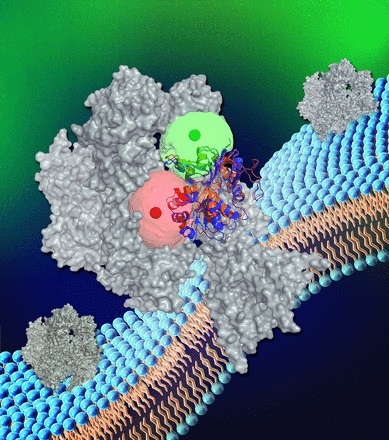
\includegraphics[width=0.5\textwidth]{figures/jbc-cover-20160729.jpg}
\caption{Sample Figure (July 29, 2016 JBC issue cover).}
\label{fig:july29cover}
\end{figure}

\begin{figure}[hbtp!]\centering
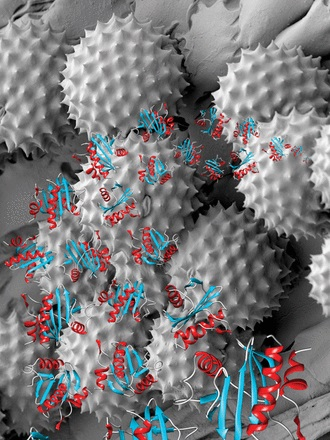
\includegraphics[width=0.5\textwidth]{figures/jbc-cover-20160722.jpg}
\caption{Sample Figure (July 22, 2016 JBC issue cover).}
\label{fig:july22cover}
\end{figure}

\begin{table}[hp!]\centering
\begin{tabular}{l r r}
Sample Heading 1 & Sample Heading 2 & Sample Heading 3\\
\hline
Data 1 & 3.8 & 0.12 \\
Data 2 & 49.2 & 0.52
\end{tabular}
\caption{A Sample Table}
\label{tab:sample}
\end{table}

References, such as \cite{Gregori2012}, must be cited in text by number only, be numbered consecutively in the order of appearance, and must include article titles, as in these examples. 

Reference management systems such as Zotero and Mendeley provide options for exporting bibliographies as Bib\TeX{} files. Bib\TeX{} is a bibliographic tool that is used with \LaTeX{} to help organize the author's references and create a bibliography. This template contains an example of such a file, \texttt{sample.bib}, which can be replaced with your own. Use the \verb|\cite| command  to create in-text citations.

\section{Discussion}

The discussion is concise (usually less than two formatted pages) and focused on the interpretation of the results. It should not repeat information in the ``Results'' section.

\section{Experimental Procedures}

The experimental procedures are brief but sufficiently complete to permit a qualified reader to repeat the experiments. Only truly new procedures should be described in detail. Previously published procedures should be referenced. Modifications of previously published procedures should not be given in detail except where necessary to repeat the work. If the study characterizes the activity of new compounds, compound structures must be provided. Quantification of gel or blot intensities must be performed with data obtained within a linear range of exposure.

\section*{acknowledgements}
Acknowledgements should include contributions from anyone who does not meet the criteria for authorship (for example, to recognize contributions from people who provided technical help, collation of data, writing assistance, acquisition of funding, or a department chairperson who provided general support), as well as any funding or other support information.

\section*{conflict of interest}
You may be asked to provide a conflict of interest statement during the submission process. Please check the journal's author guidelines for details on what to include in this section. Please ensure you liaise with all co-authors to confirm agreement with the final statement.


%% Bibliography 
\bibliography{proteomics_thesis}

\graphicalabstract{example-image-1x1}{Please check the journal's author guildines for whether a graphical abstract, key points, new findings, or other items are required for display in the Table of Contents.}

\end{document}
